% Wygenerowane przez er.py – nie edytować ręcznie.
\documentclass[tikz,border=4pt]{standalone}
\usepackage[sfdefault]{FiraSans}
\usetikzlibrary{arrows.meta}
\definecolor{head}{HTML}{23373B}
\definecolor{grid}{HTML}{C9CED6}
\definecolor{typ}{HTML}{8A929C}
\definecolor{pk}{HTML}{B7791F}
\definecolor{c-app_user}{HTML}{5B6B7F}
\definecolor{c-program}{HTML}{1F5EFF}
\definecolor{c-section}{HTML}{D9480F}
\definecolor{c-course}{HTML}{2B8A3E}
\definecolor{c-term}{HTML}{7048E8}
\definecolor{c-enrollment}{HTML}{C2255C}
\definecolor{c-room}{HTML}{8D6E63}
\definecolor{c-enrollment_round}{HTML}{0B8A7A}
\begin{document}
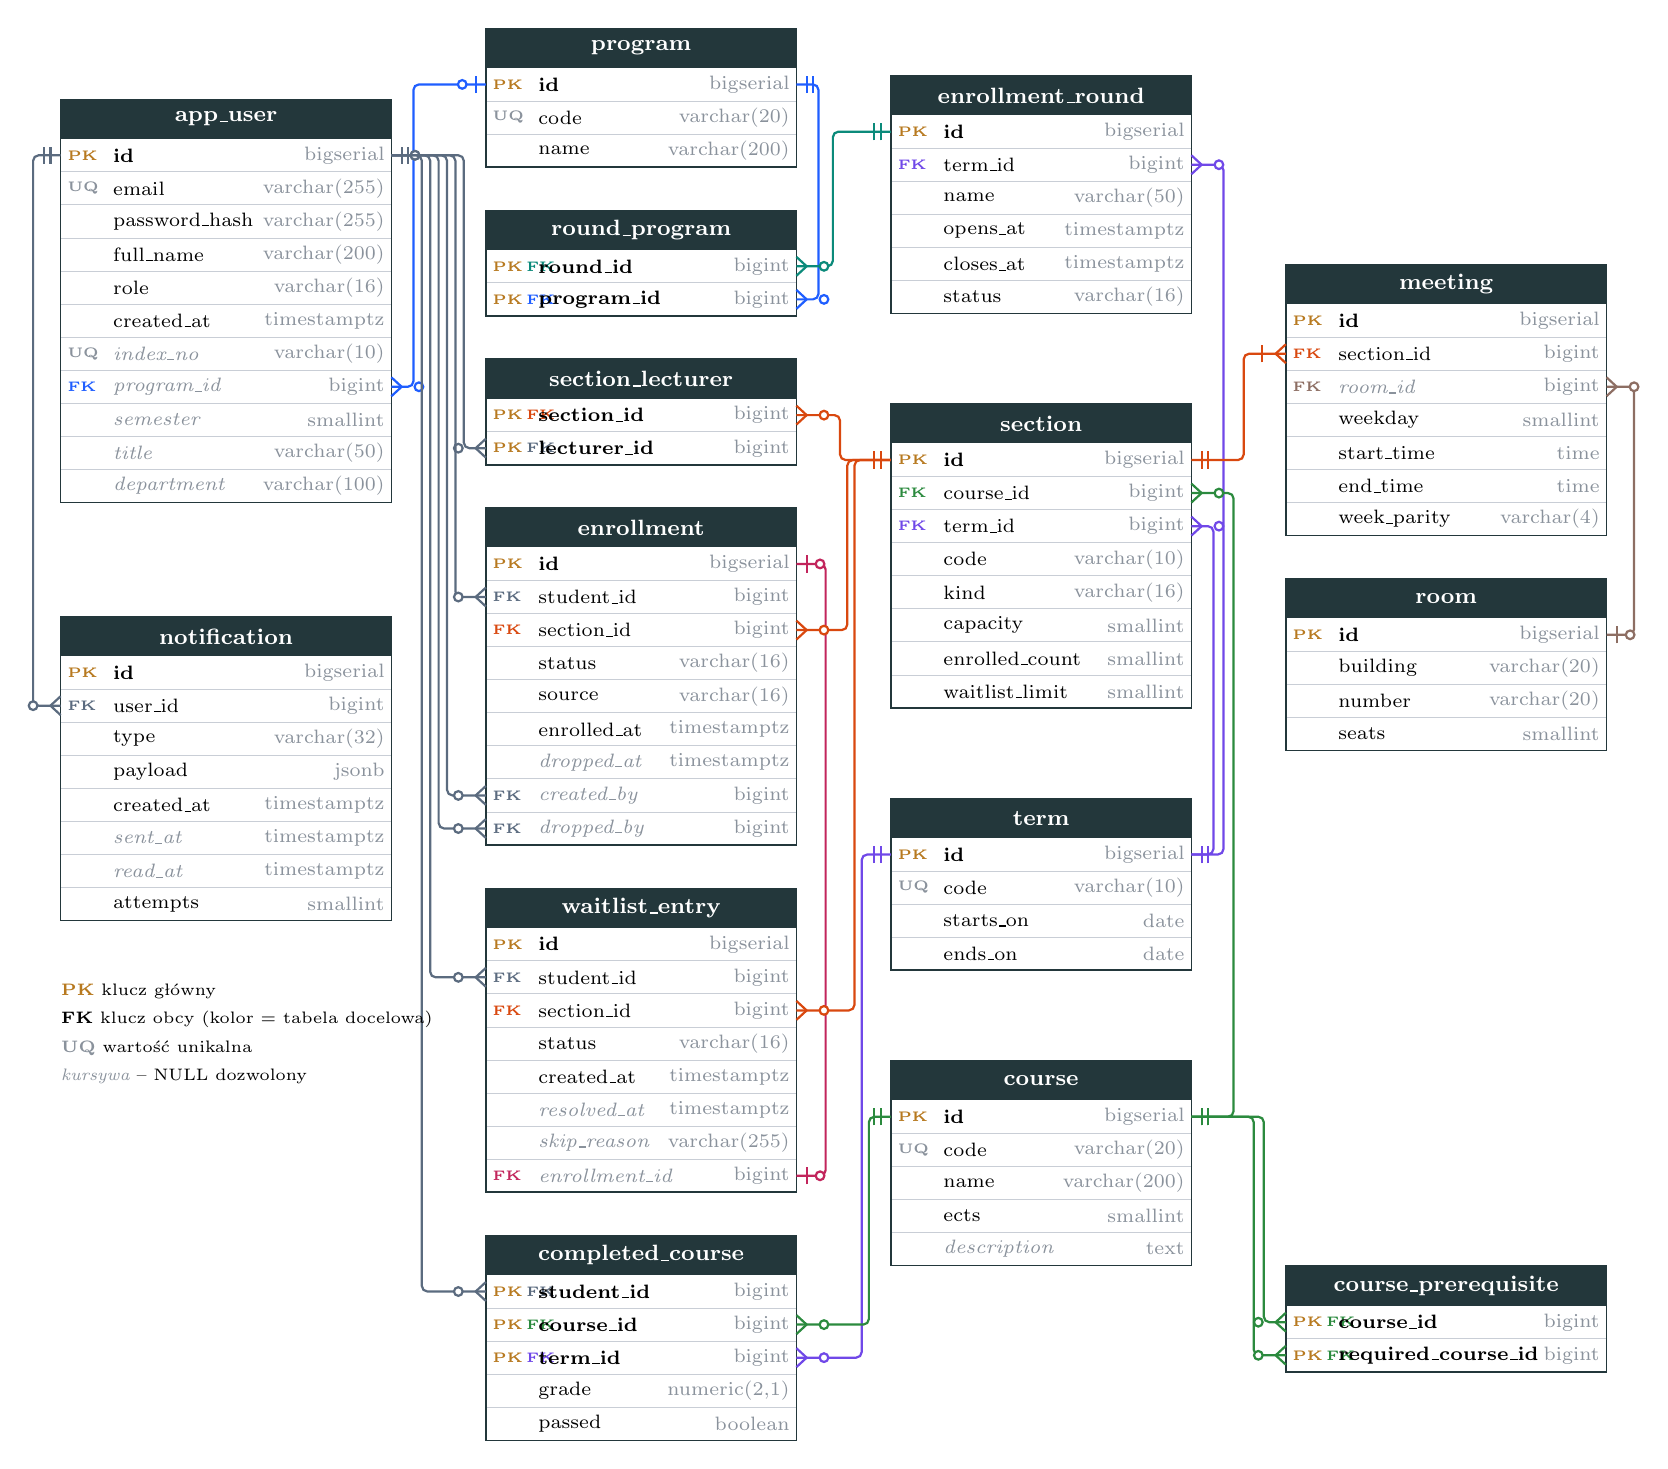
\begin{tikzpicture}[font=\fontsize{7.5}{9}\selectfont]
\fill[white] (0.000,-0.900) rectangle (4.200,-6.020);
\fill[head] (0.000,-0.900) rectangle (4.200,-1.400);
\node[white, font=\fontsize{8}{9}\selectfont\bfseries] at (2.100,-1.150) {app\_user};
\node[anchor=west, inner sep=0, font=\fontsize{5}{6}\selectfont\bfseries] at (0.080,-1.610) {\textcolor{pk}{PK}};
\node[anchor=west, inner sep=0] at (0.660,-1.610) {\textbf{id}};
\node[anchor=east, inner sep=0, text=typ] at (4.120,-1.610) {bigserial};
\draw[grid, line width=0.3pt] (0.000,-1.820) -- (4.200,-1.820);
\node[anchor=west, inner sep=0, font=\fontsize{5}{6}\selectfont\bfseries] at (0.080,-2.030) {\textcolor{typ}{UQ}};
\node[anchor=west, inner sep=0] at (0.660,-2.030) {email};
\node[anchor=east, inner sep=0, text=typ] at (4.120,-2.030) {varchar(255)};
\draw[grid, line width=0.3pt] (0.000,-2.240) -- (4.200,-2.240);
\node[anchor=west, inner sep=0, font=\fontsize{5}{6}\selectfont\bfseries] at (0.080,-2.450) {};
\node[anchor=west, inner sep=0] at (0.660,-2.450) {password\_hash};
\node[anchor=east, inner sep=0, text=typ] at (4.120,-2.450) {varchar(255)};
\draw[grid, line width=0.3pt] (0.000,-2.660) -- (4.200,-2.660);
\node[anchor=west, inner sep=0, font=\fontsize{5}{6}\selectfont\bfseries] at (0.080,-2.870) {};
\node[anchor=west, inner sep=0] at (0.660,-2.870) {full\_name};
\node[anchor=east, inner sep=0, text=typ] at (4.120,-2.870) {varchar(200)};
\draw[grid, line width=0.3pt] (0.000,-3.080) -- (4.200,-3.080);
\node[anchor=west, inner sep=0, font=\fontsize{5}{6}\selectfont\bfseries] at (0.080,-3.290) {};
\node[anchor=west, inner sep=0] at (0.660,-3.290) {role};
\node[anchor=east, inner sep=0, text=typ] at (4.120,-3.290) {varchar(16)};
\draw[grid, line width=0.3pt] (0.000,-3.500) -- (4.200,-3.500);
\node[anchor=west, inner sep=0, font=\fontsize{5}{6}\selectfont\bfseries] at (0.080,-3.710) {};
\node[anchor=west, inner sep=0] at (0.660,-3.710) {created\_at};
\node[anchor=east, inner sep=0, text=typ] at (4.120,-3.710) {timestamptz};
\draw[grid, line width=0.3pt] (0.000,-3.920) -- (4.200,-3.920);
\node[anchor=west, inner sep=0, font=\fontsize{5}{6}\selectfont\bfseries] at (0.080,-4.130) {\textcolor{typ}{UQ}};
\node[anchor=west, inner sep=0] at (0.660,-4.130) {\textcolor{typ}{\itshape index\_no}};
\node[anchor=east, inner sep=0, text=typ] at (4.120,-4.130) {varchar(10)};
\draw[grid, line width=0.3pt] (0.000,-4.340) -- (4.200,-4.340);
\node[anchor=west, inner sep=0, font=\fontsize{5}{6}\selectfont\bfseries] at (0.080,-4.550) {\textcolor{c-program}{FK}};
\node[anchor=west, inner sep=0] at (0.660,-4.550) {\textcolor{typ}{\itshape program\_id}};
\node[anchor=east, inner sep=0, text=typ] at (4.120,-4.550) {bigint};
\draw[grid, line width=0.3pt] (0.000,-4.760) -- (4.200,-4.760);
\node[anchor=west, inner sep=0, font=\fontsize{5}{6}\selectfont\bfseries] at (0.080,-4.970) {};
\node[anchor=west, inner sep=0] at (0.660,-4.970) {\textcolor{typ}{\itshape semester}};
\node[anchor=east, inner sep=0, text=typ] at (4.120,-4.970) {smallint};
\draw[grid, line width=0.3pt] (0.000,-5.180) -- (4.200,-5.180);
\node[anchor=west, inner sep=0, font=\fontsize{5}{6}\selectfont\bfseries] at (0.080,-5.390) {};
\node[anchor=west, inner sep=0] at (0.660,-5.390) {\textcolor{typ}{\itshape title}};
\node[anchor=east, inner sep=0, text=typ] at (4.120,-5.390) {varchar(50)};
\draw[grid, line width=0.3pt] (0.000,-5.600) -- (4.200,-5.600);
\node[anchor=west, inner sep=0, font=\fontsize{5}{6}\selectfont\bfseries] at (0.080,-5.810) {};
\node[anchor=west, inner sep=0] at (0.660,-5.810) {\textcolor{typ}{\itshape department}};
\node[anchor=east, inner sep=0, text=typ] at (4.120,-5.810) {varchar(100)};
\draw[head, line width=0.6pt] (0.000,-0.900) rectangle (4.200,-6.020);
\fill[white] (0.000,-7.470) rectangle (4.200,-11.330);
\fill[head] (0.000,-7.470) rectangle (4.200,-7.970);
\node[white, font=\fontsize{8}{9}\selectfont\bfseries] at (2.100,-7.720) {notification};
\node[anchor=west, inner sep=0, font=\fontsize{5}{6}\selectfont\bfseries] at (0.080,-8.180) {\textcolor{pk}{PK}};
\node[anchor=west, inner sep=0] at (0.660,-8.180) {\textbf{id}};
\node[anchor=east, inner sep=0, text=typ] at (4.120,-8.180) {bigserial};
\draw[grid, line width=0.3pt] (0.000,-8.390) -- (4.200,-8.390);
\node[anchor=west, inner sep=0, font=\fontsize{5}{6}\selectfont\bfseries] at (0.080,-8.600) {\textcolor{c-app_user}{FK}};
\node[anchor=west, inner sep=0] at (0.660,-8.600) {user\_id};
\node[anchor=east, inner sep=0, text=typ] at (4.120,-8.600) {bigint};
\draw[grid, line width=0.3pt] (0.000,-8.810) -- (4.200,-8.810);
\node[anchor=west, inner sep=0, font=\fontsize{5}{6}\selectfont\bfseries] at (0.080,-9.020) {};
\node[anchor=west, inner sep=0] at (0.660,-9.020) {type};
\node[anchor=east, inner sep=0, text=typ] at (4.120,-9.020) {varchar(32)};
\draw[grid, line width=0.3pt] (0.000,-9.230) -- (4.200,-9.230);
\node[anchor=west, inner sep=0, font=\fontsize{5}{6}\selectfont\bfseries] at (0.080,-9.440) {};
\node[anchor=west, inner sep=0] at (0.660,-9.440) {payload};
\node[anchor=east, inner sep=0, text=typ] at (4.120,-9.440) {jsonb};
\draw[grid, line width=0.3pt] (0.000,-9.650) -- (4.200,-9.650);
\node[anchor=west, inner sep=0, font=\fontsize{5}{6}\selectfont\bfseries] at (0.080,-9.860) {};
\node[anchor=west, inner sep=0] at (0.660,-9.860) {created\_at};
\node[anchor=east, inner sep=0, text=typ] at (4.120,-9.860) {timestamptz};
\draw[grid, line width=0.3pt] (0.000,-10.070) -- (4.200,-10.070);
\node[anchor=west, inner sep=0, font=\fontsize{5}{6}\selectfont\bfseries] at (0.080,-10.280) {};
\node[anchor=west, inner sep=0] at (0.660,-10.280) {\textcolor{typ}{\itshape sent\_at}};
\node[anchor=east, inner sep=0, text=typ] at (4.120,-10.280) {timestamptz};
\draw[grid, line width=0.3pt] (0.000,-10.490) -- (4.200,-10.490);
\node[anchor=west, inner sep=0, font=\fontsize{5}{6}\selectfont\bfseries] at (0.080,-10.700) {};
\node[anchor=west, inner sep=0] at (0.660,-10.700) {\textcolor{typ}{\itshape read\_at}};
\node[anchor=east, inner sep=0, text=typ] at (4.120,-10.700) {timestamptz};
\draw[grid, line width=0.3pt] (0.000,-10.910) -- (4.200,-10.910);
\node[anchor=west, inner sep=0, font=\fontsize{5}{6}\selectfont\bfseries] at (0.080,-11.120) {};
\node[anchor=west, inner sep=0] at (0.660,-11.120) {attempts};
\node[anchor=east, inner sep=0, text=typ] at (4.120,-11.120) {smallint};
\draw[head, line width=0.6pt] (0.000,-7.470) rectangle (4.200,-11.330);
\fill[white] (5.400,0.000) rectangle (9.344,-1.760);
\fill[head] (5.400,0.000) rectangle (9.344,-0.500);
\node[white, font=\fontsize{8}{9}\selectfont\bfseries] at (7.372,-0.250) {program};
\node[anchor=west, inner sep=0, font=\fontsize{5}{6}\selectfont\bfseries] at (5.480,-0.710) {\textcolor{pk}{PK}};
\node[anchor=west, inner sep=0] at (6.060,-0.710) {\textbf{id}};
\node[anchor=east, inner sep=0, text=typ] at (9.264,-0.710) {bigserial};
\draw[grid, line width=0.3pt] (5.400,-0.920) -- (9.344,-0.920);
\node[anchor=west, inner sep=0, font=\fontsize{5}{6}\selectfont\bfseries] at (5.480,-1.130) {\textcolor{typ}{UQ}};
\node[anchor=west, inner sep=0] at (6.060,-1.130) {code};
\node[anchor=east, inner sep=0, text=typ] at (9.264,-1.130) {varchar(20)};
\draw[grid, line width=0.3pt] (5.400,-1.340) -- (9.344,-1.340);
\node[anchor=west, inner sep=0, font=\fontsize{5}{6}\selectfont\bfseries] at (5.480,-1.550) {};
\node[anchor=west, inner sep=0] at (6.060,-1.550) {name};
\node[anchor=east, inner sep=0, text=typ] at (9.264,-1.550) {varchar(200)};
\draw[head, line width=0.6pt] (5.400,0.000) rectangle (9.344,-1.760);
\fill[white] (5.400,-2.310) rectangle (9.344,-3.650);
\fill[head] (5.400,-2.310) rectangle (9.344,-2.810);
\node[white, font=\fontsize{8}{9}\selectfont\bfseries] at (7.372,-2.560) {round\_program};
\node[anchor=west, inner sep=0, font=\fontsize{5}{6}\selectfont\bfseries] at (5.480,-3.020) {\textcolor{pk}{PK}\,\textcolor{c-enrollment_round}{FK}};
\node[anchor=west, inner sep=0] at (6.060,-3.020) {\textbf{round\_id}};
\node[anchor=east, inner sep=0, text=typ] at (9.264,-3.020) {bigint};
\draw[grid, line width=0.3pt] (5.400,-3.230) -- (9.344,-3.230);
\node[anchor=west, inner sep=0, font=\fontsize{5}{6}\selectfont\bfseries] at (5.480,-3.440) {\textcolor{pk}{PK}\,\textcolor{c-program}{FK}};
\node[anchor=west, inner sep=0] at (6.060,-3.440) {\textbf{program\_id}};
\node[anchor=east, inner sep=0, text=typ] at (9.264,-3.440) {bigint};
\draw[head, line width=0.6pt] (5.400,-2.310) rectangle (9.344,-3.650);
\fill[white] (5.400,-4.200) rectangle (9.344,-5.540);
\fill[head] (5.400,-4.200) rectangle (9.344,-4.700);
\node[white, font=\fontsize{8}{9}\selectfont\bfseries] at (7.372,-4.450) {section\_lecturer};
\node[anchor=west, inner sep=0, font=\fontsize{5}{6}\selectfont\bfseries] at (5.480,-4.910) {\textcolor{pk}{PK}\,\textcolor{c-section}{FK}};
\node[anchor=west, inner sep=0] at (6.060,-4.910) {\textbf{section\_id}};
\node[anchor=east, inner sep=0, text=typ] at (9.264,-4.910) {bigint};
\draw[grid, line width=0.3pt] (5.400,-5.120) -- (9.344,-5.120);
\node[anchor=west, inner sep=0, font=\fontsize{5}{6}\selectfont\bfseries] at (5.480,-5.330) {\textcolor{pk}{PK}\,\textcolor{c-app_user}{FK}};
\node[anchor=west, inner sep=0] at (6.060,-5.330) {\textbf{lecturer\_id}};
\node[anchor=east, inner sep=0, text=typ] at (9.264,-5.330) {bigint};
\draw[head, line width=0.6pt] (5.400,-4.200) rectangle (9.344,-5.540);
\fill[white] (5.400,-6.090) rectangle (9.344,-10.370);
\fill[head] (5.400,-6.090) rectangle (9.344,-6.590);
\node[white, font=\fontsize{8}{9}\selectfont\bfseries] at (7.372,-6.340) {enrollment};
\node[anchor=west, inner sep=0, font=\fontsize{5}{6}\selectfont\bfseries] at (5.480,-6.800) {\textcolor{pk}{PK}};
\node[anchor=west, inner sep=0] at (6.060,-6.800) {\textbf{id}};
\node[anchor=east, inner sep=0, text=typ] at (9.264,-6.800) {bigserial};
\draw[grid, line width=0.3pt] (5.400,-7.010) -- (9.344,-7.010);
\node[anchor=west, inner sep=0, font=\fontsize{5}{6}\selectfont\bfseries] at (5.480,-7.220) {\textcolor{c-app_user}{FK}};
\node[anchor=west, inner sep=0] at (6.060,-7.220) {student\_id};
\node[anchor=east, inner sep=0, text=typ] at (9.264,-7.220) {bigint};
\draw[grid, line width=0.3pt] (5.400,-7.430) -- (9.344,-7.430);
\node[anchor=west, inner sep=0, font=\fontsize{5}{6}\selectfont\bfseries] at (5.480,-7.640) {\textcolor{c-section}{FK}};
\node[anchor=west, inner sep=0] at (6.060,-7.640) {section\_id};
\node[anchor=east, inner sep=0, text=typ] at (9.264,-7.640) {bigint};
\draw[grid, line width=0.3pt] (5.400,-7.850) -- (9.344,-7.850);
\node[anchor=west, inner sep=0, font=\fontsize{5}{6}\selectfont\bfseries] at (5.480,-8.060) {};
\node[anchor=west, inner sep=0] at (6.060,-8.060) {status};
\node[anchor=east, inner sep=0, text=typ] at (9.264,-8.060) {varchar(16)};
\draw[grid, line width=0.3pt] (5.400,-8.270) -- (9.344,-8.270);
\node[anchor=west, inner sep=0, font=\fontsize{5}{6}\selectfont\bfseries] at (5.480,-8.480) {};
\node[anchor=west, inner sep=0] at (6.060,-8.480) {source};
\node[anchor=east, inner sep=0, text=typ] at (9.264,-8.480) {varchar(16)};
\draw[grid, line width=0.3pt] (5.400,-8.690) -- (9.344,-8.690);
\node[anchor=west, inner sep=0, font=\fontsize{5}{6}\selectfont\bfseries] at (5.480,-8.900) {};
\node[anchor=west, inner sep=0] at (6.060,-8.900) {enrolled\_at};
\node[anchor=east, inner sep=0, text=typ] at (9.264,-8.900) {timestamptz};
\draw[grid, line width=0.3pt] (5.400,-9.110) -- (9.344,-9.110);
\node[anchor=west, inner sep=0, font=\fontsize{5}{6}\selectfont\bfseries] at (5.480,-9.320) {};
\node[anchor=west, inner sep=0] at (6.060,-9.320) {\textcolor{typ}{\itshape dropped\_at}};
\node[anchor=east, inner sep=0, text=typ] at (9.264,-9.320) {timestamptz};
\draw[grid, line width=0.3pt] (5.400,-9.530) -- (9.344,-9.530);
\node[anchor=west, inner sep=0, font=\fontsize{5}{6}\selectfont\bfseries] at (5.480,-9.740) {\textcolor{c-app_user}{FK}};
\node[anchor=west, inner sep=0] at (6.060,-9.740) {\textcolor{typ}{\itshape created\_by}};
\node[anchor=east, inner sep=0, text=typ] at (9.264,-9.740) {bigint};
\draw[grid, line width=0.3pt] (5.400,-9.950) -- (9.344,-9.950);
\node[anchor=west, inner sep=0, font=\fontsize{5}{6}\selectfont\bfseries] at (5.480,-10.160) {\textcolor{c-app_user}{FK}};
\node[anchor=west, inner sep=0] at (6.060,-10.160) {\textcolor{typ}{\itshape dropped\_by}};
\node[anchor=east, inner sep=0, text=typ] at (9.264,-10.160) {bigint};
\draw[head, line width=0.6pt] (5.400,-6.090) rectangle (9.344,-10.370);
\fill[white] (5.400,-10.920) rectangle (9.344,-14.780);
\fill[head] (5.400,-10.920) rectangle (9.344,-11.420);
\node[white, font=\fontsize{8}{9}\selectfont\bfseries] at (7.372,-11.170) {waitlist\_entry};
\node[anchor=west, inner sep=0, font=\fontsize{5}{6}\selectfont\bfseries] at (5.480,-11.630) {\textcolor{pk}{PK}};
\node[anchor=west, inner sep=0] at (6.060,-11.630) {\textbf{id}};
\node[anchor=east, inner sep=0, text=typ] at (9.264,-11.630) {bigserial};
\draw[grid, line width=0.3pt] (5.400,-11.840) -- (9.344,-11.840);
\node[anchor=west, inner sep=0, font=\fontsize{5}{6}\selectfont\bfseries] at (5.480,-12.050) {\textcolor{c-app_user}{FK}};
\node[anchor=west, inner sep=0] at (6.060,-12.050) {student\_id};
\node[anchor=east, inner sep=0, text=typ] at (9.264,-12.050) {bigint};
\draw[grid, line width=0.3pt] (5.400,-12.260) -- (9.344,-12.260);
\node[anchor=west, inner sep=0, font=\fontsize{5}{6}\selectfont\bfseries] at (5.480,-12.470) {\textcolor{c-section}{FK}};
\node[anchor=west, inner sep=0] at (6.060,-12.470) {section\_id};
\node[anchor=east, inner sep=0, text=typ] at (9.264,-12.470) {bigint};
\draw[grid, line width=0.3pt] (5.400,-12.680) -- (9.344,-12.680);
\node[anchor=west, inner sep=0, font=\fontsize{5}{6}\selectfont\bfseries] at (5.480,-12.890) {};
\node[anchor=west, inner sep=0] at (6.060,-12.890) {status};
\node[anchor=east, inner sep=0, text=typ] at (9.264,-12.890) {varchar(16)};
\draw[grid, line width=0.3pt] (5.400,-13.100) -- (9.344,-13.100);
\node[anchor=west, inner sep=0, font=\fontsize{5}{6}\selectfont\bfseries] at (5.480,-13.310) {};
\node[anchor=west, inner sep=0] at (6.060,-13.310) {created\_at};
\node[anchor=east, inner sep=0, text=typ] at (9.264,-13.310) {timestamptz};
\draw[grid, line width=0.3pt] (5.400,-13.520) -- (9.344,-13.520);
\node[anchor=west, inner sep=0, font=\fontsize{5}{6}\selectfont\bfseries] at (5.480,-13.730) {};
\node[anchor=west, inner sep=0] at (6.060,-13.730) {\textcolor{typ}{\itshape resolved\_at}};
\node[anchor=east, inner sep=0, text=typ] at (9.264,-13.730) {timestamptz};
\draw[grid, line width=0.3pt] (5.400,-13.940) -- (9.344,-13.940);
\node[anchor=west, inner sep=0, font=\fontsize{5}{6}\selectfont\bfseries] at (5.480,-14.150) {};
\node[anchor=west, inner sep=0] at (6.060,-14.150) {\textcolor{typ}{\itshape skip\_reason}};
\node[anchor=east, inner sep=0, text=typ] at (9.264,-14.150) {varchar(255)};
\draw[grid, line width=0.3pt] (5.400,-14.360) -- (9.344,-14.360);
\node[anchor=west, inner sep=0, font=\fontsize{5}{6}\selectfont\bfseries] at (5.480,-14.570) {\textcolor{c-enrollment}{FK}};
\node[anchor=west, inner sep=0] at (6.060,-14.570) {\textcolor{typ}{\itshape enrollment\_id}};
\node[anchor=east, inner sep=0, text=typ] at (9.264,-14.570) {bigint};
\draw[head, line width=0.6pt] (5.400,-10.920) rectangle (9.344,-14.780);
\fill[white] (5.400,-15.330) rectangle (9.344,-17.930);
\fill[head] (5.400,-15.330) rectangle (9.344,-15.830);
\node[white, font=\fontsize{8}{9}\selectfont\bfseries] at (7.372,-15.580) {completed\_course};
\node[anchor=west, inner sep=0, font=\fontsize{5}{6}\selectfont\bfseries] at (5.480,-16.040) {\textcolor{pk}{PK}\,\textcolor{c-app_user}{FK}};
\node[anchor=west, inner sep=0] at (6.060,-16.040) {\textbf{student\_id}};
\node[anchor=east, inner sep=0, text=typ] at (9.264,-16.040) {bigint};
\draw[grid, line width=0.3pt] (5.400,-16.250) -- (9.344,-16.250);
\node[anchor=west, inner sep=0, font=\fontsize{5}{6}\selectfont\bfseries] at (5.480,-16.460) {\textcolor{pk}{PK}\,\textcolor{c-course}{FK}};
\node[anchor=west, inner sep=0] at (6.060,-16.460) {\textbf{course\_id}};
\node[anchor=east, inner sep=0, text=typ] at (9.264,-16.460) {bigint};
\draw[grid, line width=0.3pt] (5.400,-16.670) -- (9.344,-16.670);
\node[anchor=west, inner sep=0, font=\fontsize{5}{6}\selectfont\bfseries] at (5.480,-16.880) {\textcolor{pk}{PK}\,\textcolor{c-term}{FK}};
\node[anchor=west, inner sep=0] at (6.060,-16.880) {\textbf{term\_id}};
\node[anchor=east, inner sep=0, text=typ] at (9.264,-16.880) {bigint};
\draw[grid, line width=0.3pt] (5.400,-17.090) -- (9.344,-17.090);
\node[anchor=west, inner sep=0, font=\fontsize{5}{6}\selectfont\bfseries] at (5.480,-17.300) {};
\node[anchor=west, inner sep=0] at (6.060,-17.300) {grade};
\node[anchor=east, inner sep=0, text=typ] at (9.264,-17.300) {numeric(2,1)};
\draw[grid, line width=0.3pt] (5.400,-17.510) -- (9.344,-17.510);
\node[anchor=west, inner sep=0, font=\fontsize{5}{6}\selectfont\bfseries] at (5.480,-17.720) {};
\node[anchor=west, inner sep=0] at (6.060,-17.720) {passed};
\node[anchor=east, inner sep=0, text=typ] at (9.264,-17.720) {boolean};
\draw[head, line width=0.6pt] (5.400,-15.330) rectangle (9.344,-17.930);
\fill[white] (10.544,-0.600) rectangle (14.360,-3.620);
\fill[head] (10.544,-0.600) rectangle (14.360,-1.100);
\node[white, font=\fontsize{8}{9}\selectfont\bfseries] at (12.452,-0.850) {enrollment\_round};
\node[anchor=west, inner sep=0, font=\fontsize{5}{6}\selectfont\bfseries] at (10.624,-1.310) {\textcolor{pk}{PK}};
\node[anchor=west, inner sep=0] at (11.204,-1.310) {\textbf{id}};
\node[anchor=east, inner sep=0, text=typ] at (14.280,-1.310) {bigserial};
\draw[grid, line width=0.3pt] (10.544,-1.520) -- (14.360,-1.520);
\node[anchor=west, inner sep=0, font=\fontsize{5}{6}\selectfont\bfseries] at (10.624,-1.730) {\textcolor{c-term}{FK}};
\node[anchor=west, inner sep=0] at (11.204,-1.730) {term\_id};
\node[anchor=east, inner sep=0, text=typ] at (14.280,-1.730) {bigint};
\draw[grid, line width=0.3pt] (10.544,-1.940) -- (14.360,-1.940);
\node[anchor=west, inner sep=0, font=\fontsize{5}{6}\selectfont\bfseries] at (10.624,-2.150) {};
\node[anchor=west, inner sep=0] at (11.204,-2.150) {name};
\node[anchor=east, inner sep=0, text=typ] at (14.280,-2.150) {varchar(50)};
\draw[grid, line width=0.3pt] (10.544,-2.360) -- (14.360,-2.360);
\node[anchor=west, inner sep=0, font=\fontsize{5}{6}\selectfont\bfseries] at (10.624,-2.570) {};
\node[anchor=west, inner sep=0] at (11.204,-2.570) {opens\_at};
\node[anchor=east, inner sep=0, text=typ] at (14.280,-2.570) {timestamptz};
\draw[grid, line width=0.3pt] (10.544,-2.780) -- (14.360,-2.780);
\node[anchor=west, inner sep=0, font=\fontsize{5}{6}\selectfont\bfseries] at (10.624,-2.990) {};
\node[anchor=west, inner sep=0] at (11.204,-2.990) {closes\_at};
\node[anchor=east, inner sep=0, text=typ] at (14.280,-2.990) {timestamptz};
\draw[grid, line width=0.3pt] (10.544,-3.200) -- (14.360,-3.200);
\node[anchor=west, inner sep=0, font=\fontsize{5}{6}\selectfont\bfseries] at (10.624,-3.410) {};
\node[anchor=west, inner sep=0] at (11.204,-3.410) {status};
\node[anchor=east, inner sep=0, text=typ] at (14.280,-3.410) {varchar(16)};
\draw[head, line width=0.6pt] (10.544,-0.600) rectangle (14.360,-3.620);
\fill[white] (10.544,-4.770) rectangle (14.360,-8.630);
\fill[head] (10.544,-4.770) rectangle (14.360,-5.270);
\node[white, font=\fontsize{8}{9}\selectfont\bfseries] at (12.452,-5.020) {section};
\node[anchor=west, inner sep=0, font=\fontsize{5}{6}\selectfont\bfseries] at (10.624,-5.480) {\textcolor{pk}{PK}};
\node[anchor=west, inner sep=0] at (11.204,-5.480) {\textbf{id}};
\node[anchor=east, inner sep=0, text=typ] at (14.280,-5.480) {bigserial};
\draw[grid, line width=0.3pt] (10.544,-5.690) -- (14.360,-5.690);
\node[anchor=west, inner sep=0, font=\fontsize{5}{6}\selectfont\bfseries] at (10.624,-5.900) {\textcolor{c-course}{FK}};
\node[anchor=west, inner sep=0] at (11.204,-5.900) {course\_id};
\node[anchor=east, inner sep=0, text=typ] at (14.280,-5.900) {bigint};
\draw[grid, line width=0.3pt] (10.544,-6.110) -- (14.360,-6.110);
\node[anchor=west, inner sep=0, font=\fontsize{5}{6}\selectfont\bfseries] at (10.624,-6.320) {\textcolor{c-term}{FK}};
\node[anchor=west, inner sep=0] at (11.204,-6.320) {term\_id};
\node[anchor=east, inner sep=0, text=typ] at (14.280,-6.320) {bigint};
\draw[grid, line width=0.3pt] (10.544,-6.530) -- (14.360,-6.530);
\node[anchor=west, inner sep=0, font=\fontsize{5}{6}\selectfont\bfseries] at (10.624,-6.740) {};
\node[anchor=west, inner sep=0] at (11.204,-6.740) {code};
\node[anchor=east, inner sep=0, text=typ] at (14.280,-6.740) {varchar(10)};
\draw[grid, line width=0.3pt] (10.544,-6.950) -- (14.360,-6.950);
\node[anchor=west, inner sep=0, font=\fontsize{5}{6}\selectfont\bfseries] at (10.624,-7.160) {};
\node[anchor=west, inner sep=0] at (11.204,-7.160) {kind};
\node[anchor=east, inner sep=0, text=typ] at (14.280,-7.160) {varchar(16)};
\draw[grid, line width=0.3pt] (10.544,-7.370) -- (14.360,-7.370);
\node[anchor=west, inner sep=0, font=\fontsize{5}{6}\selectfont\bfseries] at (10.624,-7.580) {};
\node[anchor=west, inner sep=0] at (11.204,-7.580) {capacity};
\node[anchor=east, inner sep=0, text=typ] at (14.280,-7.580) {smallint};
\draw[grid, line width=0.3pt] (10.544,-7.790) -- (14.360,-7.790);
\node[anchor=west, inner sep=0, font=\fontsize{5}{6}\selectfont\bfseries] at (10.624,-8.000) {};
\node[anchor=west, inner sep=0] at (11.204,-8.000) {enrolled\_count};
\node[anchor=east, inner sep=0, text=typ] at (14.280,-8.000) {smallint};
\draw[grid, line width=0.3pt] (10.544,-8.210) -- (14.360,-8.210);
\node[anchor=west, inner sep=0, font=\fontsize{5}{6}\selectfont\bfseries] at (10.624,-8.420) {};
\node[anchor=west, inner sep=0] at (11.204,-8.420) {waitlist\_limit};
\node[anchor=east, inner sep=0, text=typ] at (14.280,-8.420) {smallint};
\draw[head, line width=0.6pt] (10.544,-4.770) rectangle (14.360,-8.630);
\fill[white] (10.544,-9.780) rectangle (14.360,-11.960);
\fill[head] (10.544,-9.780) rectangle (14.360,-10.280);
\node[white, font=\fontsize{8}{9}\selectfont\bfseries] at (12.452,-10.030) {term};
\node[anchor=west, inner sep=0, font=\fontsize{5}{6}\selectfont\bfseries] at (10.624,-10.490) {\textcolor{pk}{PK}};
\node[anchor=west, inner sep=0] at (11.204,-10.490) {\textbf{id}};
\node[anchor=east, inner sep=0, text=typ] at (14.280,-10.490) {bigserial};
\draw[grid, line width=0.3pt] (10.544,-10.700) -- (14.360,-10.700);
\node[anchor=west, inner sep=0, font=\fontsize{5}{6}\selectfont\bfseries] at (10.624,-10.910) {\textcolor{typ}{UQ}};
\node[anchor=west, inner sep=0] at (11.204,-10.910) {code};
\node[anchor=east, inner sep=0, text=typ] at (14.280,-10.910) {varchar(10)};
\draw[grid, line width=0.3pt] (10.544,-11.120) -- (14.360,-11.120);
\node[anchor=west, inner sep=0, font=\fontsize{5}{6}\selectfont\bfseries] at (10.624,-11.330) {};
\node[anchor=west, inner sep=0] at (11.204,-11.330) {starts\_on};
\node[anchor=east, inner sep=0, text=typ] at (14.280,-11.330) {date};
\draw[grid, line width=0.3pt] (10.544,-11.540) -- (14.360,-11.540);
\node[anchor=west, inner sep=0, font=\fontsize{5}{6}\selectfont\bfseries] at (10.624,-11.750) {};
\node[anchor=west, inner sep=0] at (11.204,-11.750) {ends\_on};
\node[anchor=east, inner sep=0, text=typ] at (14.280,-11.750) {date};
\draw[head, line width=0.6pt] (10.544,-9.780) rectangle (14.360,-11.960);
\fill[white] (10.544,-13.110) rectangle (14.360,-15.710);
\fill[head] (10.544,-13.110) rectangle (14.360,-13.610);
\node[white, font=\fontsize{8}{9}\selectfont\bfseries] at (12.452,-13.360) {course};
\node[anchor=west, inner sep=0, font=\fontsize{5}{6}\selectfont\bfseries] at (10.624,-13.820) {\textcolor{pk}{PK}};
\node[anchor=west, inner sep=0] at (11.204,-13.820) {\textbf{id}};
\node[anchor=east, inner sep=0, text=typ] at (14.280,-13.820) {bigserial};
\draw[grid, line width=0.3pt] (10.544,-14.030) -- (14.360,-14.030);
\node[anchor=west, inner sep=0, font=\fontsize{5}{6}\selectfont\bfseries] at (10.624,-14.240) {\textcolor{typ}{UQ}};
\node[anchor=west, inner sep=0] at (11.204,-14.240) {code};
\node[anchor=east, inner sep=0, text=typ] at (14.280,-14.240) {varchar(20)};
\draw[grid, line width=0.3pt] (10.544,-14.450) -- (14.360,-14.450);
\node[anchor=west, inner sep=0, font=\fontsize{5}{6}\selectfont\bfseries] at (10.624,-14.660) {};
\node[anchor=west, inner sep=0] at (11.204,-14.660) {name};
\node[anchor=east, inner sep=0, text=typ] at (14.280,-14.660) {varchar(200)};
\draw[grid, line width=0.3pt] (10.544,-14.870) -- (14.360,-14.870);
\node[anchor=west, inner sep=0, font=\fontsize{5}{6}\selectfont\bfseries] at (10.624,-15.080) {};
\node[anchor=west, inner sep=0] at (11.204,-15.080) {ects};
\node[anchor=east, inner sep=0, text=typ] at (14.280,-15.080) {smallint};
\draw[grid, line width=0.3pt] (10.544,-15.290) -- (14.360,-15.290);
\node[anchor=west, inner sep=0, font=\fontsize{5}{6}\selectfont\bfseries] at (10.624,-15.500) {};
\node[anchor=west, inner sep=0] at (11.204,-15.500) {\textcolor{typ}{\itshape description}};
\node[anchor=east, inner sep=0, text=typ] at (14.280,-15.500) {text};
\draw[head, line width=0.6pt] (10.544,-13.110) rectangle (14.360,-15.710);
\fill[white] (15.560,-3.000) rectangle (19.632,-6.440);
\fill[head] (15.560,-3.000) rectangle (19.632,-3.500);
\node[white, font=\fontsize{8}{9}\selectfont\bfseries] at (17.596,-3.250) {meeting};
\node[anchor=west, inner sep=0, font=\fontsize{5}{6}\selectfont\bfseries] at (15.640,-3.710) {\textcolor{pk}{PK}};
\node[anchor=west, inner sep=0] at (16.220,-3.710) {\textbf{id}};
\node[anchor=east, inner sep=0, text=typ] at (19.552,-3.710) {bigserial};
\draw[grid, line width=0.3pt] (15.560,-3.920) -- (19.632,-3.920);
\node[anchor=west, inner sep=0, font=\fontsize{5}{6}\selectfont\bfseries] at (15.640,-4.130) {\textcolor{c-section}{FK}};
\node[anchor=west, inner sep=0] at (16.220,-4.130) {section\_id};
\node[anchor=east, inner sep=0, text=typ] at (19.552,-4.130) {bigint};
\draw[grid, line width=0.3pt] (15.560,-4.340) -- (19.632,-4.340);
\node[anchor=west, inner sep=0, font=\fontsize{5}{6}\selectfont\bfseries] at (15.640,-4.550) {\textcolor{c-room}{FK}};
\node[anchor=west, inner sep=0] at (16.220,-4.550) {\textcolor{typ}{\itshape room\_id}};
\node[anchor=east, inner sep=0, text=typ] at (19.552,-4.550) {bigint};
\draw[grid, line width=0.3pt] (15.560,-4.760) -- (19.632,-4.760);
\node[anchor=west, inner sep=0, font=\fontsize{5}{6}\selectfont\bfseries] at (15.640,-4.970) {};
\node[anchor=west, inner sep=0] at (16.220,-4.970) {weekday};
\node[anchor=east, inner sep=0, text=typ] at (19.552,-4.970) {smallint};
\draw[grid, line width=0.3pt] (15.560,-5.180) -- (19.632,-5.180);
\node[anchor=west, inner sep=0, font=\fontsize{5}{6}\selectfont\bfseries] at (15.640,-5.390) {};
\node[anchor=west, inner sep=0] at (16.220,-5.390) {start\_time};
\node[anchor=east, inner sep=0, text=typ] at (19.552,-5.390) {time};
\draw[grid, line width=0.3pt] (15.560,-5.600) -- (19.632,-5.600);
\node[anchor=west, inner sep=0, font=\fontsize{5}{6}\selectfont\bfseries] at (15.640,-5.810) {};
\node[anchor=west, inner sep=0] at (16.220,-5.810) {end\_time};
\node[anchor=east, inner sep=0, text=typ] at (19.552,-5.810) {time};
\draw[grid, line width=0.3pt] (15.560,-6.020) -- (19.632,-6.020);
\node[anchor=west, inner sep=0, font=\fontsize{5}{6}\selectfont\bfseries] at (15.640,-6.230) {};
\node[anchor=west, inner sep=0] at (16.220,-6.230) {week\_parity};
\node[anchor=east, inner sep=0, text=typ] at (19.552,-6.230) {varchar(4)};
\draw[head, line width=0.6pt] (15.560,-3.000) rectangle (19.632,-6.440);
\fill[white] (15.560,-6.990) rectangle (19.632,-9.170);
\fill[head] (15.560,-6.990) rectangle (19.632,-7.490);
\node[white, font=\fontsize{8}{9}\selectfont\bfseries] at (17.596,-7.240) {room};
\node[anchor=west, inner sep=0, font=\fontsize{5}{6}\selectfont\bfseries] at (15.640,-7.700) {\textcolor{pk}{PK}};
\node[anchor=west, inner sep=0] at (16.220,-7.700) {\textbf{id}};
\node[anchor=east, inner sep=0, text=typ] at (19.552,-7.700) {bigserial};
\draw[grid, line width=0.3pt] (15.560,-7.910) -- (19.632,-7.910);
\node[anchor=west, inner sep=0, font=\fontsize{5}{6}\selectfont\bfseries] at (15.640,-8.120) {};
\node[anchor=west, inner sep=0] at (16.220,-8.120) {building};
\node[anchor=east, inner sep=0, text=typ] at (19.552,-8.120) {varchar(20)};
\draw[grid, line width=0.3pt] (15.560,-8.330) -- (19.632,-8.330);
\node[anchor=west, inner sep=0, font=\fontsize{5}{6}\selectfont\bfseries] at (15.640,-8.540) {};
\node[anchor=west, inner sep=0] at (16.220,-8.540) {number};
\node[anchor=east, inner sep=0, text=typ] at (19.552,-8.540) {varchar(20)};
\draw[grid, line width=0.3pt] (15.560,-8.750) -- (19.632,-8.750);
\node[anchor=west, inner sep=0, font=\fontsize{5}{6}\selectfont\bfseries] at (15.640,-8.960) {};
\node[anchor=west, inner sep=0] at (16.220,-8.960) {seats};
\node[anchor=east, inner sep=0, text=typ] at (19.552,-8.960) {smallint};
\draw[head, line width=0.6pt] (15.560,-6.990) rectangle (19.632,-9.170);
\fill[white] (15.560,-15.720) rectangle (19.632,-17.060);
\fill[head] (15.560,-15.720) rectangle (19.632,-16.220);
\node[white, font=\fontsize{8}{9}\selectfont\bfseries] at (17.596,-15.970) {course\_prerequisite};
\node[anchor=west, inner sep=0, font=\fontsize{5}{6}\selectfont\bfseries] at (15.640,-16.430) {\textcolor{pk}{PK}\,\textcolor{c-course}{FK}};
\node[anchor=west, inner sep=0] at (16.220,-16.430) {\textbf{course\_id}};
\node[anchor=east, inner sep=0, text=typ] at (19.552,-16.430) {bigint};
\draw[grid, line width=0.3pt] (15.560,-16.640) -- (19.632,-16.640);
\node[anchor=west, inner sep=0, font=\fontsize{5}{6}\selectfont\bfseries] at (15.640,-16.850) {\textcolor{pk}{PK}\,\textcolor{c-course}{FK}};
\node[anchor=west, inner sep=0] at (16.220,-16.850) {\textbf{required\_course\_id}};
\node[anchor=east, inner sep=0, text=typ] at (19.552,-16.850) {bigint};
\draw[head, line width=0.6pt] (15.560,-15.720) rectangle (19.632,-17.060);
\draw[c-app_user, line width=0.8pt, rounded corners=2pt] (0.000,-8.600) -- (-0.350,-8.600) -- (-0.350,-1.610) -- (0.000,-1.610);
\draw[c-app_user, line width=0.8pt] (-0.130,-8.600) -- (0.000,-8.480) (-0.130,-8.600) -- (0.000,-8.720);
\draw[c-app_user, line width=0.8pt, fill=white] (-0.350,-8.600) circle (0.055);
\draw[c-app_user, line width=0.8pt] (-0.130,-1.720) -- (-0.130,-1.500);
\draw[c-app_user, line width=0.8pt] (-0.210,-1.720) -- (-0.210,-1.500);
\draw[c-program, line width=0.8pt, rounded corners=2pt] (4.200,-4.550) -- (4.480,-4.550) -- (4.480,-0.710) -- (5.400,-0.710);
\draw[c-program, line width=0.8pt] (4.330,-4.550) -- (4.200,-4.430) (4.330,-4.550) -- (4.200,-4.670);
\draw[c-program, line width=0.8pt, fill=white] (4.550,-4.550) circle (0.055);
\draw[c-program, line width=0.8pt] (5.270,-0.820) -- (5.270,-0.600);
\draw[c-program, line width=0.8pt, fill=white] (5.100,-0.710) circle (0.055);
\draw[c-app_user, line width=0.8pt, rounded corners=2pt] (5.400,-5.330) -- (5.120,-5.330) -- (5.120,-1.610) -- (4.200,-1.610);
\draw[c-app_user, line width=0.8pt] (5.270,-5.330) -- (5.400,-5.210) (5.270,-5.330) -- (5.400,-5.450);
\draw[c-app_user, line width=0.8pt, fill=white] (5.050,-5.330) circle (0.055);
\draw[c-app_user, line width=0.8pt] (4.330,-1.720) -- (4.330,-1.500);
\draw[c-app_user, line width=0.8pt] (4.410,-1.720) -- (4.410,-1.500);
\draw[c-app_user, line width=0.8pt, rounded corners=2pt] (5.400,-7.220) -- (5.013,-7.220) -- (5.013,-1.610) -- (4.200,-1.610);
\draw[c-app_user, line width=0.8pt] (5.270,-7.220) -- (5.400,-7.100) (5.270,-7.220) -- (5.400,-7.340);
\draw[c-app_user, line width=0.8pt, fill=white] (5.050,-7.220) circle (0.055);
\draw[c-app_user, line width=0.8pt] (4.330,-1.720) -- (4.330,-1.500);
\draw[c-app_user, line width=0.8pt] (4.410,-1.720) -- (4.410,-1.500);
\draw[c-app_user, line width=0.8pt, rounded corners=2pt] (5.400,-9.740) -- (4.907,-9.740) -- (4.907,-1.610) -- (4.200,-1.610);
\draw[c-app_user, line width=0.8pt] (5.270,-9.740) -- (5.400,-9.620) (5.270,-9.740) -- (5.400,-9.860);
\draw[c-app_user, line width=0.8pt, fill=white] (5.050,-9.740) circle (0.055);
\draw[c-app_user, line width=0.8pt] (4.330,-1.720) -- (4.330,-1.500);
\draw[c-app_user, line width=0.8pt, fill=white] (4.500,-1.610) circle (0.055);
\draw[c-app_user, line width=0.8pt, rounded corners=2pt] (5.400,-10.160) -- (4.800,-10.160) -- (4.800,-1.610) -- (4.200,-1.610);
\draw[c-app_user, line width=0.8pt] (5.270,-10.160) -- (5.400,-10.040) (5.270,-10.160) -- (5.400,-10.280);
\draw[c-app_user, line width=0.8pt, fill=white] (5.050,-10.160) circle (0.055);
\draw[c-app_user, line width=0.8pt] (4.330,-1.720) -- (4.330,-1.500);
\draw[c-app_user, line width=0.8pt, fill=white] (4.500,-1.610) circle (0.055);
\draw[c-app_user, line width=0.8pt, rounded corners=2pt] (5.400,-12.050) -- (4.693,-12.050) -- (4.693,-1.610) -- (4.200,-1.610);
\draw[c-app_user, line width=0.8pt] (5.270,-12.050) -- (5.400,-11.930) (5.270,-12.050) -- (5.400,-12.170);
\draw[c-app_user, line width=0.8pt, fill=white] (5.050,-12.050) circle (0.055);
\draw[c-app_user, line width=0.8pt] (4.330,-1.720) -- (4.330,-1.500);
\draw[c-app_user, line width=0.8pt] (4.410,-1.720) -- (4.410,-1.500);
\draw[c-app_user, line width=0.8pt, rounded corners=2pt] (5.400,-16.040) -- (4.587,-16.040) -- (4.587,-1.610) -- (4.200,-1.610);
\draw[c-app_user, line width=0.8pt] (5.270,-16.040) -- (5.400,-15.920) (5.270,-16.040) -- (5.400,-16.160);
\draw[c-app_user, line width=0.8pt, fill=white] (5.050,-16.040) circle (0.055);
\draw[c-app_user, line width=0.8pt] (4.330,-1.720) -- (4.330,-1.500);
\draw[c-app_user, line width=0.8pt] (4.410,-1.720) -- (4.410,-1.500);
\draw[c-program, line width=0.8pt, rounded corners=2pt] (9.344,-3.440) -- (9.624,-3.440) -- (9.624,-0.710) -- (9.344,-0.710);
\draw[c-program, line width=0.8pt] (9.474,-3.440) -- (9.344,-3.320) (9.474,-3.440) -- (9.344,-3.560);
\draw[c-program, line width=0.8pt, fill=white] (9.694,-3.440) circle (0.055);
\draw[c-program, line width=0.8pt] (9.474,-0.820) -- (9.474,-0.600);
\draw[c-program, line width=0.8pt] (9.554,-0.820) -- (9.554,-0.600);
\draw[c-enrollment_round, line width=0.8pt, rounded corners=2pt] (9.344,-3.020) -- (9.807,-3.020) -- (9.807,-1.310) -- (10.544,-1.310);
\draw[c-enrollment_round, line width=0.8pt] (9.474,-3.020) -- (9.344,-2.900) (9.474,-3.020) -- (9.344,-3.140);
\draw[c-enrollment_round, line width=0.8pt, fill=white] (9.694,-3.020) circle (0.055);
\draw[c-enrollment_round, line width=0.8pt] (10.414,-1.420) -- (10.414,-1.200);
\draw[c-enrollment_round, line width=0.8pt] (10.334,-1.420) -- (10.334,-1.200);
\draw[c-enrollment, line width=0.8pt, rounded corners=2pt] (9.344,-14.570) -- (9.715,-14.570) -- (9.715,-6.800) -- (9.344,-6.800);
\draw[c-enrollment, line width=0.8pt] (9.474,-14.680) -- (9.474,-14.460);
\draw[c-enrollment, line width=0.8pt, fill=white] (9.644,-14.570) circle (0.055);
\draw[c-enrollment, line width=0.8pt] (9.474,-6.910) -- (9.474,-6.690);
\draw[c-enrollment, line width=0.8pt, fill=white] (9.644,-6.800) circle (0.055);
\draw[c-section, line width=0.8pt, rounded corners=2pt] (9.344,-4.910) -- (9.898,-4.910) -- (9.898,-5.480) -- (10.544,-5.480);
\draw[c-section, line width=0.8pt] (9.474,-4.910) -- (9.344,-4.790) (9.474,-4.910) -- (9.344,-5.030);
\draw[c-section, line width=0.8pt, fill=white] (9.694,-4.910) circle (0.055);
\draw[c-section, line width=0.8pt] (10.414,-5.590) -- (10.414,-5.370);
\draw[c-section, line width=0.8pt] (10.334,-5.590) -- (10.334,-5.370);
\draw[c-section, line width=0.8pt, rounded corners=2pt] (9.344,-7.640) -- (9.990,-7.640) -- (9.990,-5.480) -- (10.544,-5.480);
\draw[c-section, line width=0.8pt] (9.474,-7.640) -- (9.344,-7.520) (9.474,-7.640) -- (9.344,-7.760);
\draw[c-section, line width=0.8pt, fill=white] (9.694,-7.640) circle (0.055);
\draw[c-section, line width=0.8pt] (10.414,-5.590) -- (10.414,-5.370);
\draw[c-section, line width=0.8pt] (10.334,-5.590) -- (10.334,-5.370);
\draw[c-section, line width=0.8pt, rounded corners=2pt] (9.344,-12.470) -- (10.081,-12.470) -- (10.081,-5.480) -- (10.544,-5.480);
\draw[c-section, line width=0.8pt] (9.474,-12.470) -- (9.344,-12.350) (9.474,-12.470) -- (9.344,-12.590);
\draw[c-section, line width=0.8pt, fill=white] (9.694,-12.470) circle (0.055);
\draw[c-section, line width=0.8pt] (10.414,-5.590) -- (10.414,-5.370);
\draw[c-section, line width=0.8pt] (10.334,-5.590) -- (10.334,-5.370);
\draw[c-term, line width=0.8pt, rounded corners=2pt] (9.344,-16.880) -- (10.173,-16.880) -- (10.173,-10.490) -- (10.544,-10.490);
\draw[c-term, line width=0.8pt] (9.474,-16.880) -- (9.344,-16.760) (9.474,-16.880) -- (9.344,-17.000);
\draw[c-term, line width=0.8pt, fill=white] (9.694,-16.880) circle (0.055);
\draw[c-term, line width=0.8pt] (10.414,-10.600) -- (10.414,-10.380);
\draw[c-term, line width=0.8pt] (10.334,-10.600) -- (10.334,-10.380);
\draw[c-course, line width=0.8pt, rounded corners=2pt] (9.344,-16.460) -- (10.264,-16.460) -- (10.264,-13.820) -- (10.544,-13.820);
\draw[c-course, line width=0.8pt] (9.474,-16.460) -- (9.344,-16.340) (9.474,-16.460) -- (9.344,-16.580);
\draw[c-course, line width=0.8pt, fill=white] (9.694,-16.460) circle (0.055);
\draw[c-course, line width=0.8pt] (10.414,-13.930) -- (10.414,-13.710);
\draw[c-course, line width=0.8pt] (10.334,-13.930) -- (10.334,-13.710);
\draw[c-term, line width=0.8pt, rounded corners=2pt] (14.360,-1.730) -- (14.768,-1.730) -- (14.768,-10.490) -- (14.360,-10.490);
\draw[c-term, line width=0.8pt] (14.490,-1.730) -- (14.360,-1.610) (14.490,-1.730) -- (14.360,-1.850);
\draw[c-term, line width=0.8pt, fill=white] (14.710,-1.730) circle (0.055);
\draw[c-term, line width=0.8pt] (14.490,-10.600) -- (14.490,-10.380);
\draw[c-term, line width=0.8pt] (14.570,-10.600) -- (14.570,-10.380);
\draw[c-term, line width=0.8pt, rounded corners=2pt] (14.360,-6.320) -- (14.640,-6.320) -- (14.640,-10.490) -- (14.360,-10.490);
\draw[c-term, line width=0.8pt] (14.490,-6.320) -- (14.360,-6.200) (14.490,-6.320) -- (14.360,-6.440);
\draw[c-term, line width=0.8pt, fill=white] (14.710,-6.320) circle (0.055);
\draw[c-term, line width=0.8pt] (14.490,-10.600) -- (14.490,-10.380);
\draw[c-term, line width=0.8pt] (14.570,-10.600) -- (14.570,-10.380);
\draw[c-course, line width=0.8pt, rounded corners=2pt] (14.360,-5.900) -- (14.896,-5.900) -- (14.896,-13.820) -- (14.360,-13.820);
\draw[c-course, line width=0.8pt] (14.490,-5.900) -- (14.360,-5.780) (14.490,-5.900) -- (14.360,-6.020);
\draw[c-course, line width=0.8pt, fill=white] (14.710,-5.900) circle (0.055);
\draw[c-course, line width=0.8pt] (14.490,-13.930) -- (14.490,-13.710);
\draw[c-course, line width=0.8pt] (14.570,-13.930) -- (14.570,-13.710);
\draw[c-section, line width=0.8pt, rounded corners=2pt] (15.560,-4.130) -- (15.024,-4.130) -- (15.024,-5.480) -- (14.360,-5.480);
\draw[c-section, line width=0.8pt] (15.430,-4.130) -- (15.560,-4.010) (15.430,-4.130) -- (15.560,-4.250);
\draw[c-section, line width=0.8pt] (15.260,-4.240) -- (15.260,-4.020);
\draw[c-section, line width=0.8pt] (14.490,-5.590) -- (14.490,-5.370);
\draw[c-section, line width=0.8pt] (14.570,-5.590) -- (14.570,-5.370);
\draw[c-course, line width=0.8pt, rounded corners=2pt] (15.560,-16.430) -- (15.280,-16.430) -- (15.280,-13.820) -- (14.360,-13.820);
\draw[c-course, line width=0.8pt] (15.430,-16.430) -- (15.560,-16.310) (15.430,-16.430) -- (15.560,-16.550);
\draw[c-course, line width=0.8pt, fill=white] (15.210,-16.430) circle (0.055);
\draw[c-course, line width=0.8pt] (14.490,-13.930) -- (14.490,-13.710);
\draw[c-course, line width=0.8pt] (14.570,-13.930) -- (14.570,-13.710);
\draw[c-course, line width=0.8pt, rounded corners=2pt] (15.560,-16.850) -- (15.152,-16.850) -- (15.152,-13.820) -- (14.360,-13.820);
\draw[c-course, line width=0.8pt] (15.430,-16.850) -- (15.560,-16.730) (15.430,-16.850) -- (15.560,-16.970);
\draw[c-course, line width=0.8pt, fill=white] (15.210,-16.850) circle (0.055);
\draw[c-course, line width=0.8pt] (14.490,-13.930) -- (14.490,-13.710);
\draw[c-course, line width=0.8pt] (14.570,-13.930) -- (14.570,-13.710);
\draw[c-room, line width=0.8pt, rounded corners=2pt] (19.632,-4.550) -- (19.982,-4.550) -- (19.982,-7.700) -- (19.632,-7.700);
\draw[c-room, line width=0.8pt] (19.762,-4.550) -- (19.632,-4.430) (19.762,-4.550) -- (19.632,-4.670);
\draw[c-room, line width=0.8pt, fill=white] (19.982,-4.550) circle (0.055);
\draw[c-room, line width=0.8pt] (19.762,-7.810) -- (19.762,-7.590);
\draw[c-room, line width=0.8pt, fill=white] (19.932,-7.700) circle (0.055);
\node[anchor=west, inner sep=0, font=\fontsize{6.5}{8}\selectfont] at (0.000,-12.230) {\textcolor{pk}{\bfseries PK} klucz główny};
\node[anchor=west, inner sep=0, font=\fontsize{6.5}{8}\selectfont] at (0.000,-12.590) {\bfseries FK\mdseries{} klucz obcy (kolor = tabela docelowa)};
\node[anchor=west, inner sep=0, font=\fontsize{6.5}{8}\selectfont] at (0.000,-12.950) {\textcolor{typ}{\bfseries UQ} wartość unikalna};
\node[anchor=west, inner sep=0, font=\fontsize{6.5}{8}\selectfont] at (0.000,-13.310) {\textcolor{typ}{\itshape kursywa} -- NULL dozwolony};
\end{tikzpicture}
\end{document}
